%!TEX root = /Users/louis/Documents/PhD/Deliverables/Thesis/thesis.tex

\section{Metamodel-Independent Syntax}
\label{sec:mmi_syntax}
Section~\ref{subsec:modelling_framework_characteristics} discussed the way in which modelling frameworks implicitly enforce conformance. Because of this, modelling frameworks cannot be used to load non-conformant models, and provide little support for checking the conformance of a model with other metamodels or other versions of a metamodel. In Section~\ref{sec:requirements_identification}, these concerns lead to the identification of the following requirement: \emph{This thesis must investigate the extension of existing modelling frameworks to support the loading of non-conformant models and conformance checking of models against other metamodels.}

This section describes the way in which existing modelling frameworks load and store models using a metamodel-specific syntax. An alternative storage representation is motivated by highlighting the problems that a metamodel-specific syntax poses for managing and automating co-evolution. The way in which automatic consistency checking can be performed using the alternative storage representation is demonstrated. The work presented in this section has been published in \cite{rose09enhanced}.


\subsection{Model Storage Representation}
Throughout a model-driven development process, modelling frameworks are used to load and store models. XML Metadata Interchange (XMI) \cite{xmi}, the OMG standard for exchanging MOF-based models, is the canonical model representation used by many contemporary modelling frameworks. XMI specifies the way in which models should be represented in XML.

An XMI document defines one or more namespaces from which type information is drawn. For example, XMI itself provides a namespace for specifying the version of XMI being used. Metamodels are referenced via namespaces, allowing the specification of elements that instantiate metamodel types.

As discussed in Section~\ref{subsec:modelling_framework_characteristics}, modelling frameworks bind a model to its metamodel using the underlying programming language. The metamodel defines the way in which model elements will be bound, and frequently, binding is strongly-typed: each metamodel type is mapped to a corresponding type in the underlying programming language.

Listing~\ref{lst:xmi} shows XMI for an exemplar model conforming to a metamodel that defines \texttt{Person} as a metaclass with three features: a string-valued \texttt{name}, an optional reference to a \texttt{Person}, \texttt{mother}, and another optional reference to a \texttt{Person}, \texttt{father}.

\begin{lstlisting}[caption=Exemplar person model in XMI, label=lst:xmi, language=XML]
<?xml version="1.0" encoding="ASCII"?>
<xmi:XMI xmi:version="2.0" xmlns:xmi="http://www.omg.org/XMI" xmlns:families="http://www.cs.york.ac.uk/families">
	<families:Person xmi:id="_xNSb8KfZEd,0dNl1iq3EdQ" name="Franz" mother="_6ef33ff010b31df8a39080" father="_F520cDaa0jN,i10s8xZp2a" />
	<families:Person xmi:id="_6ef33ff010b31df8a39080" name="Julie" />
	<families:Person xmi:id="_F520cDaa0jN,i10s8xZp2a" name="Hermann" />
</xmi:XMI>
\end{lstlisting}

The model shown in Listing~\ref{lst:xmi} contains three \texttt{Person}s, Franz, Julie and Hermann. Julie is the mother and Hermann is the father of Franz. The mothers and fathers of Julie and Hermann are not specified. On line 2, the XMI document specifies that the families namespace will be used to refer to types defined by the metamodel with the identifier: \url{http://www.cs.york.ac.uk/families}. Each person defines an XMI ID (a universally unique identifier), and a name. The IDs are used for inter-element references, such as for the values of the mother and father features.

Binding a model element involves instantiating, in the underlying programming language, the metamodel type, and populating the attributes of the instantiated object with values that correspond to those specified in the model. Because an XMI document refers to metamodel types and features by name, binding fails when a model does not conform to its metamodel. 


\subsection{Binding to a generic metamodel}
\label{subsec:binding}
For situations when a model does not conform to its metamodel, this thesis proposes an alternative deserialisation mechanism, which binds a model to a \emph{generic} metamodel. A generic metamodel reflects the characteristics of the metamodelling language and consequently every model conforms to the generic metamodel. Figure~\ref{fig:slot_model} shows a minimal version of a generic metamodel for MOF. Model elements are bound to \texttt{Object}, data values to \texttt{Slot}.

\begin{figure}[htbp]
  \centering
  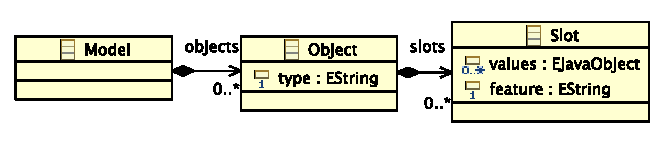
\includegraphics[width=3.3in]{5.Implementation/slot_model.pdf}
  \caption{A generic metamodel.}
  \label{fig:slot_model}
\end{figure}

Using the metamodel in Figure~\ref{fig:slot_model} in conjunction with MOF, conformance constraints can be expressed, as shown below. A minimal subset of MOF is shown in Figure~\ref{fig:minimal_mof}.

\begin{figure}[htbp]
  \centering
  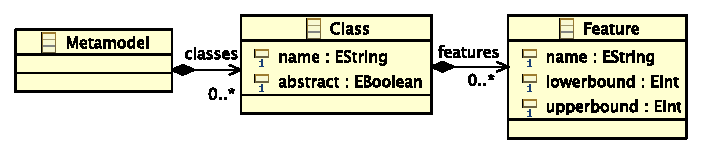
\includegraphics[width=3.3in]{5.Implementation/mof.pdf}
  \caption{Minimal MOF metamodel.}
  \label{fig:minimal_mof}
\end{figure}

The following constraints between metamodels (e.g. instances of MOF, Figure~\ref{fig:minimal_mof}) and models represented with a generic metamodel (e.g. instances of Figure~\ref{fig:slot_model}) can be used to express conformance:

\begin{enumerate}
	\item Each object's type must be the name of some non-abstract metamodel class.
	\item Each object must specify a slot for each mandatory feature of its type.
	\item Each slot's feature must be the name of a metamodel feature. That metamodel feature must belong to the slot's owning object's type.
	\item Each slot must be multiplicity-compatible with its feature. More specifically, each slot must contain at least as many values as its feature's lower bound, and at most as many values as its feature's upper bound.
  \item Each slot must be type-compatible with its feature.
\end{enumerate}

The way in which type-compatibility is checked depends on the way in which the modelling framework is implemented, and on its underlying programming language. EMF, for example, is implemented in Java and exposes some services for checking the type compatibility of model data with metamodel features. All metamodel features are typed and their types provide methods for determining the underlying programming language representation. Type compatibility checks can be implemented using these methods.

Conformance constraints vary over modelling languages. For example, Ecore, the modelling language of EMF, is similar to but not the same as MOF. For example, metamodel features defined in Ecore can be marked as transient (not stored to disk) and unchangeable (read-only). In EMF, extra conformance constraints are required which restrict the feature value of slots to only non-transient, changeable features.


\subsection{Example}
\label{subsec:mmi_syntax_example}
By binding a model not to the underlying programming languages types defined in its metamodel but to the generic metamodel presented in Figure~\ref{fig:slot_model}, conformance can be checked using the above constraints. Binding the exemplar XMI in Listing~\ref{lst:xmi} to the generic metamodel shown in Figure~\ref{fig:slot_model} produces three Objects, all with type ``Person''. Each class object contains a slot whose feature is name, one with the value ``Franz'', one with the value ``Julie'' and the other with the value ``Hermann''. The object containing the slot with value ``Franz'' contains two further slots: one whose feature is mother and whose value is a reference\footnote{The generic metamodel used in this thesis implements reference values using the proxy design pattern \cite{gamma95patterns}.} to the object that contains the name slot with the value ``Julie'' and one whose feature is father and whose value is a reference to the object containing ``Hermann''. A UML object diagram for this instantiation of the generic metamodel is shown in Figure~\ref{fig:generic_binding}. Instances of object (slot) are shaded grey (white).

\begin{figure}[htbp]
  \centering
  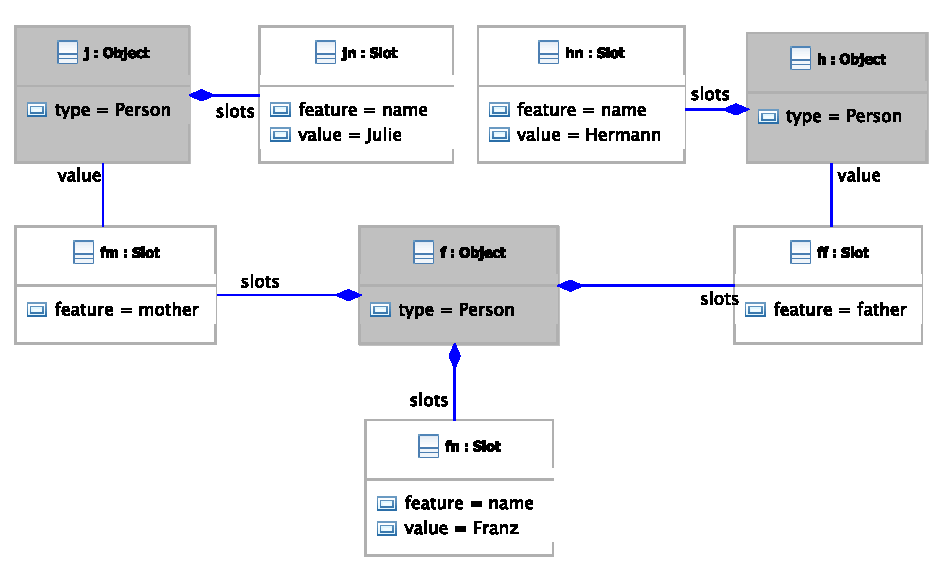
\includegraphics[width=4in]{5.Implementation/GenericBinding.pdf}
  \caption{Exemplar instantiation of generic metamodel.}
  \label{fig:generic_binding}
\end{figure}

After binding to the generic metamodel, the conformance of a model can be checked against any metamodel. Suppose the metamodel used to construct the XMI shown in Figure~\ref{fig:slot_model} has now evolved. The mother and father references have been removed, and replaced by a unifying parents reference. Conformance checking for the object representing Franz will fail because it defines slots for features ``mother'' and ``father'', which are no longer defined for the metamodel class ``Person''. More specifically, the model element representing Franz does not satisfy conformance constraint 4 from Section~\ref{subsec:binding}, which states that: each slot's feature must be the name of a metamodel feature. That metamodel feature must belong to the slot's owning object's type. 

\subsection{Applications}
As this section has shown, binding to a metamodel independent syntax is an alternative model deserialisation mechanism that can be used when a model no longer conforms to its metamodel and to check the conformance of a model with any metamodel. The metamodel independent syntax described in this section is used throughout this chapter to support other structures and processes for co-evolution.

In Section~\ref{sec:notation}, a textual modelling notation is integrated with the metamodel independent model representation discussed here. In Section~\ref{sec:flock}, a domain-specific language for migration uses metamodel independent syntax to perform partial migration by producing models that conform to a generic metamodel rather than their evolved metamodel.

One of the model migration tools discussed in Section~\ref{sec:analyis_of_languages_used_for_migration}, COPE \cite{herrmannsdoerfer09cope}, proposes a model migration language that manipulates models via a metamodel-independent syntax. Some of the strengths and weaknesses of that approach and using a metamodel-independent syntax in that context are described in Sections~\ref{subsubsec:cope} and~\ref{subsec:analysis}.


\subsubsection{Automatic Consistency Checking}
\label{subsec:automatic_checking}
In addition to the applications outlined above, a metamodel independent syntax is particularly useful during metamodel installation. As discussed in Section~\ref{subsec:modelling_framework_characteristics}, metamodel developers do not have access to downstream models. Consequently, instances of a metamodel may become non-conformant after a new version of a metamodel plug-in is installed. By default, an EMF metamodel plug-in does not check conformance during plug-in installation and non-conformant models are only detected when the user attempts to load them.

To enable conformance checking as part of metamodel installation in EMF, the binding to a generic metamodel discussed above has been integrated with Concordance \cite{rose10concordance} in joint work with Dimitrios S. Kolovos, a lecturer in this department, Nicholas Drivalos, a research associate in this department and James R. Williams, a research student in this department.

Concordance provides a light-weight and efficient mechanism for resolving inter-model references, including the references between models and their metamodels. Concordance can be used to efficiently determine the instances of a metamodel, which is otherwise only possible with a brute force search of a development workspace.

The integration work involved extending Concordance such that, after the installation of a metamodel plug-in, models that conform to any previous version of the metamodel are identified. Those models are checked for conformance with the new metamodel. As such, conformance checking occurs automatically and during metamodel installation. Conformance problems are detected and reported immediately, rather than when the user next attempts to load an affected model. By integrating conformance checking with Concordance, improved scalability is achieved, as demonstrated in \cite{rose10concordance}. 